% =============================================================================
%  Machine Learning for Petroleum Engineers Using Python
%  Módulo 7 · Clase 3: Titanic de Punta a Punta --- y la Red que Ve
%  SLB Ecuador | UDLA
%
%  Compilar: pdflatex -shell-escape presentacion.tex (x2 para refs)
% =============================================================================
\documentclass[aspectratio=169, 11pt]{beamer}

% ── Codificación y lenguaje ──────────────────────────────────────────────────
\usepackage[T1]{fontenc}
\usepackage[utf8]{inputenc}
\usepackage[spanish,es-noshorthands]{babel}

% ── Fuentes ──────────────────────────────────────────────────────────────────
\usepackage{FiraSans}
\usepackage{FiraMono}
\renewcommand{\familydefault}{\sfdefault}

% ── Gráficos y diagramas ────────────────────────────────────────────────────
\usepackage{graphicx}
\usepackage{tikz}
\usetikzlibrary{arrows.meta, positioning, shapes.geometric, calc, fit, decorations.pathreplacing}
\usepackage{fontawesome5}

% ── Código fuente ────────────────────────────────────────────────────────────
\usepackage{minted}
\usepackage{tcolorbox}
\tcbuselibrary{minted, skins, breakable}

% ── Tablas y utilidades ──────────────────────────────────────────────────────
\usepackage{amsmath}
\usepackage{colortbl}
\usepackage{booktabs}
\usepackage{multicol}
\usepackage{hyperref}
\usepackage{calc}

% =============================================================================
%  PALETA DE COLORES (rojo UDLA + variantes)
% =============================================================================
\definecolor{arcaRed}{HTML}{C82B40}
\definecolor{arcaDark}{HTML}{6B1525}
\definecolor{udlaCrimson}{HTML}{A31545}
\definecolor{arcaGray}{HTML}{F5F5F5}
\definecolor{arcaLightGray}{HTML}{EBEBEB}
\definecolor{textDark}{HTML}{2D2D2D}
\definecolor{textMuted}{HTML}{6B7280}
\definecolor{codeGreen}{HTML}{16A34A}
\definecolor{codeBlue}{HTML}{2563EB}
\definecolor{codeOrange}{HTML}{EA580C}
\definecolor{slbBlue}{HTML}{0014DC}
\definecolor{terminalBg}{HTML}{0F172A}
\definecolor{terminalGreen}{HTML}{86EFAC}
\definecolor{terminalMuted}{HTML}{94A3B8}
\definecolor{codeBg}{HTML}{FAFAFA}

% =============================================================================
%  CONFIGURACIÓN DEL TEMA BEAMER
% =============================================================================
\usetheme{default}
\usecolortheme{default}

\setbeamertemplate{navigation symbols}{}
\setbeamertemplate{footline}{}
\setbeamertemplate{headline}{}

\setbeamercolor{normal text}{fg=textDark}
\setbeamercolor{frametitle}{fg=arcaRed, bg=white}
\setbeamercolor{title}{fg=white}
\setbeamercolor{subtitle}{fg=white!85}
\setbeamercolor{author}{fg=white!80}
\setbeamercolor{date}{fg=white!70}
\setbeamercolor{item}{fg=arcaRed}
\setbeamercolor{subitem}{fg=arcaDark}
\setbeamercolor{block title}{fg=white, bg=arcaRed}
\setbeamercolor{block body}{fg=textDark, bg=arcaGray}
\setbeamercolor{block title alerted}{fg=white, bg=codeOrange}
\setbeamercolor{block body alerted}{fg=textDark, bg=arcaGray}
\setbeamercolor{block title example}{fg=white, bg=codeGreen}
\setbeamercolor{block body example}{fg=textDark, bg=arcaGray}
\setbeamercolor{section in toc}{fg=arcaDark}

\setbeamerfont{frametitle}{size=\Large, series=\bfseries}
\setbeamerfont{title}{size=\huge, series=\bfseries}
\setbeamerfont{subtitle}{size=\large}
\setbeamerfont{author}{size=\normalsize}
\setbeamerfont{date}{size=\small}
\setbeamerfont{block title}{size=\normalsize, series=\bfseries}
\setbeamerfont{footnote}{size=\tiny}

\setbeamertemplate{itemize item}{\scriptsize\raise1.5pt\hbox{\color{arcaRed}$\blacktriangleright$}}
\setbeamertemplate{itemize subitem}{\scriptsize\raise1pt\hbox{\color{arcaDark}$\bullet$}}
\setbeamertemplate{enumerate items}[default]
\setbeamercolor{enumerate item}{fg=arcaRed}

% =============================================================================
%  HEADER
% =============================================================================
\setbeamertemplate{headline}{%
  \begin{tikzpicture}[remember picture, overlay]
    \fill[arcaDark] (current page.north west) rectangle
      ([yshift=-0.7cm]current page.north east);
    \node[anchor=west, inner sep=0pt] at
      ([xshift=0.6cm, yshift=-0.35cm]current page.north west)
      {
\includegraphics[height=0.45cm]{../logo_udla_white.png}};
    \node[anchor=east, inner sep=0pt] at
      ([xshift=-0.6cm, yshift=-0.35cm]current page.north east)
      {
\includegraphics[height=0.42cm]{../SLB_white.png}};
  \end{tikzpicture}%
  \vspace{0.7cm}%
}

% =============================================================================
%  FOOTER
% =============================================================================
\setbeamertemplate{footline}{%
  \begin{tikzpicture}[remember picture, overlay]
    \draw[arcaLightGray, line width=0.4pt]
      ([yshift=0.55cm, xshift=0.6cm]current page.south west) --
      ([yshift=0.55cm, xshift=-0.6cm]current page.south east);
    \node[anchor=south, font=\tiny\color{textMuted}] at
      ([yshift=0.15cm]current page.south)
      {Machine Learning for Petroleum Engineers Using Python \(\cdot\) SLB Ecuador};
    \node[anchor=south east, font=\scriptsize\bfseries\color{arcaRed}] at
      ([xshift=-0.6cm, yshift=0.15cm]current page.south east)
      {\insertframenumber};
  \end{tikzpicture}%
}

% =============================================================================
%  FRAMETITLE personalizado con línea roja
% =============================================================================
\setbeamertemplate{frametitle}{%
  \vspace{0.25cm}%
  \usebeamerfont{frametitle}\usebeamercolor[fg]{frametitle}\insertframetitle%
  \par\vspace{2pt}%
  \begin{tikzpicture}
    \fill[arcaRed] (0,0) rectangle (3cm, 1.5pt);
    \fill[arcaLightGray] (3cm,0) rectangle (\textwidth, 0.5pt);
  \end{tikzpicture}%
  \vspace{0.1cm}%
}

% =============================================================================
%  ESTILO DE BLOQUES DE CÓDIGO (minted + tcolorbox)
% =============================================================================
\newtcblisting{pyblock}[1][]{%
  listing engine=minted,
  minted language=python,
  minted style=xcode,
  minted options={
    fontsize=\small,
    linenos=false,
    breaklines=true,
    python3=true
  },
  enhanced,
  colback=codeBg,
  colframe=arcaRed,
  left=8pt,
  right=6pt,
  top=5pt,
  bottom=5pt,
  boxrule=0pt,
  leftrule=3pt,
  arc=3pt,
  listing only,
  title={\hspace{-2pt}\faPython\hspace{5pt}Python},
  fonttitle=\scriptsize\bfseries,
  colbacktitle=arcaRed,
  coltitle=white,
  attach boxed title to top left={xshift=8pt, yshift=-7pt},
  boxed title style={
    arc=2pt, boxrule=0pt,
    top=1.5pt, bottom=1.5pt, left=6pt, right=6pt
  },
  drop fuzzy shadow=black!12,
  #1
}

\newtcblisting{outputblock}[1][]{%
  listing engine=minted,
  minted language=text,
  minted style=bw,
  minted options={
    fontsize=\small,
    breaklines=true,
    formatcom=\color{terminalGreen}
  },
  enhanced,
  colback=terminalBg,
  colframe=terminalBg,
  coltext=terminalGreen,
  left=10pt, right=6pt, top=5pt, bottom=5pt,
  boxrule=0pt,
  arc=3pt,
  listing only,
  title={\hspace{-2pt}\faTerminal\hspace{5pt}Output},
  fonttitle=\scriptsize\bfseries,
  colbacktitle=terminalGreen!85!black,
  coltitle=terminalBg,
  attach boxed title to top left={xshift=8pt, yshift=-7pt},
  boxed title style={
    arc=2pt, boxrule=0pt,
    top=1.5pt, bottom=1.5pt, left=6pt, right=6pt
  },
  #1
}

% =============================================================================
%  SECTION DIVIDERS
% =============================================================================
\newcommand{\sectionframe}[2]{%
  \begingroup
    \setbeamertemplate{headline}{}
    \setbeamertemplate{footline}{}
    \setbeamertemplate{navigation symbols}{}
    \begin{frame}[plain, noframenumbering]
      \begin{tikzpicture}[remember picture, overlay]
        \fill[arcaRed] (current page.south west) rectangle (current page.north east);
        \node[anchor=center, text=white, font=\Huge\bfseries, text width=15cm,
              align=center] at ([yshift=0.5cm]current page.center)
              {\hyphenpenalty=10000\exhyphenpenalty=10000 #1};
        \node[anchor=center, text=white!80, font=\large, text width=10cm,
              align=center] at ([yshift=-0.8cm]current page.center) {#2};
      \end{tikzpicture}
    \end{frame}
  \endgroup
}

% =============================================================================
%  METADATOS
% =============================================================================
\title{Machine Learning for Petroleum Engineers\\Using Python}
\subtitle{Módulo 7 · Clase 3: Titanic de Punta a Punta --- y la Red que Ve}
\author{Carlos Enrique Mosquera Trujillo}
\date{2026}

% =============================================================================
%  DOCUMENTO
% =============================================================================
% =============================================================================
%  DOCUMENTO
% =============================================================================
% =============================================================================
%  Cajas de PROMPT (se copian al agente) y de ENCARGO.
% =============================================================================
\newtcolorbox{prompt}[1][]{%
  colback=arcaGray, colframe=arcaDark, boxrule=0pt, leftrule=3.5pt,
  arc=3pt, left=8pt, right=8pt, top=6pt, bottom=6pt,
  fontupper=\ttfamily\scriptsize\color{textMuted},
  title={\hspace{-2pt}\faRobot\hspace{5pt}#1},
  fonttitle=\scriptsize\bfseries\sffamily,
  colbacktitle=arcaDark, coltitle=white,
  attach boxed title to top left={xshift=8pt, yshift=-7pt},
  boxed title style={arc=2pt, boxrule=0pt,
    top=1.5pt, bottom=1.5pt, left=6pt, right=6pt}}

\begin{document}
% ── PORTADA ──────────────────────────────────────────────────────────────────
{
\setbeamertemplate{headline}{}
\setbeamertemplate{footline}{}
\begin{frame}[plain, noframenumbering]
  \begin{tikzpicture}[remember picture, overlay]
    \fill[white] (current page.south west) rectangle (current page.north east);
    \fill[arcaRed] (current page.north west) rectangle ([yshift=-0.35cm]current page.north east);
    \fill[arcaDark] (current page.south west) rectangle ([yshift=0.35cm]current page.south east);
    \fill[arcaRed]
      ([xshift=1.1cm, yshift=-0.35cm]current page.north west) rectangle
      ([xshift=1.15cm, yshift=0.35cm]current page.south west);
    \node[anchor=north west, inner sep=0pt] at
      ([xshift=1.8cm, yshift=-1.2cm]current page.north west)
      {
\includegraphics[height=1.6cm]{../logo_udla.png}};
    \node[anchor=north east, inner sep=0pt] at
      ([xshift=-1.5cm, yshift=-1.2cm]current page.north east)
      {
\includegraphics[height=1.5cm]{../SLB.png}};
    \node[anchor=center, text=arcaDark, text width=14.5cm, align=center] at
      ([yshift=0.95cm]current page.center) {
        {\LARGE\bfseries Machine Learning for Petroleum Engineers}\\[8pt]
        {\LARGE\bfseries Using Python}
      };
    \fill[arcaRed]
      ([yshift=-0.35cm, xshift=-3.2cm]current page.center) rectangle
      ([yshift=-0.28cm, xshift=3.2cm]current page.center);
    \node[anchor=center, text=arcaRed, font=\large, text width=13.5cm, align=center] at
      ([yshift=-1.3cm]current page.center) {
        Módulo 7 · Clase 3\\[3pt]
        Titanic de Punta a Punta --- y la Red que Ve
      };
    \node[anchor=center, text=textMuted, font=\normalsize] at
      ([yshift=-2.5cm]current page.center) {
        {\color{arcaRed}\faUser}\hspace{6pt}Carlos Enrique Mosquera Trujillo
        \hspace{16pt}
        {\color{arcaRed}\faIndustry}\hspace{4pt}SLB Ecuador
      };
  \end{tikzpicture}
\end{frame}
}

% ── DÓNDE ESTAMOS ────────────────────────────────────────────────────────────
\begin{frame}[shrink=5]{Dónde Estamos: Dos Actos}
  \vspace{-2pt}
  \begin{columns}[T]
    \begin{column}{0.48\textwidth}
      {\small\color{arcaDark}\bfseries\faTheaterMasks\hspace{5pt}Acto 1 --- resuelto conmigo:}
      \vspace{4pt}
      {\footnotesize\color{textMuted}
      \begin{itemize}\setlength{\itemsep}{4pt}
        \item[{\color{arcaRed}\scriptsize\faArrowRight}]
          \textbf{Titanic de punta a punta}: EDA, limpieza, comparación de
          modelos, probabilidades, explicabilidad y app
        \item[{\color{arcaRed}\scriptsize\faArrowRight}]
          Es \textbf{la plantilla de su proyecto} --- lo que se entrega el
          jueves, con su dato
      \end{itemize}}
    \end{column}
    \begin{column}{0.48\textwidth}
      {\small\color{arcaDark}\bfseries\faBrain\hspace{5pt}Acto 2 --- construido por ustedes:}
      \vspace{4pt}
      {\footnotesize\color{textMuted}
      \begin{itemize}\setlength{\itemsep}{4pt}
        \item[{\color{codeGreen}\scriptsize\faCheck}]
          Su primera \textbf{red neuronal} --- y la pregunta honesta de si
          le gana al boosting
        \item[{\color{codeGreen}\scriptsize\faCheck}]
          La \textbf{no linealidad}, vista con los ojos
        \item[{\color{codeGreen}\scriptsize\faCheck}]
          Una red que \textbf{lee dígitos} --- y una que \textbf{ve fotos}
          sin que la entrenemos
      \end{itemize}}
    \end{column}
  \end{columns}
  \vspace{6pt}
  \begin{tcolorbox}[colback=arcaGray, colframe=arcaDark, boxrule=0pt,
    leftrule=3pt, arc=3pt, left=8pt, right=8pt, top=4pt, bottom=4pt]
    {\scriptsize\color{textMuted}
     El Acto 2 va \textbf{guiado como la Clase 1}: la carga del dato viene
     dada, el prompt está listo para pegar, y el código lo construye el
     agente dirigido por ustedes. \textbf{Proyecto:} equipos de hasta 3,
     entrega hasta el jueves de la próxima semana.}
  \end{tcolorbox}
\end{frame}

% ═════════════════════════════════════════════════════════════════════════════
\sectionframe{Acto 1 · Titanic de Punta a Punta}{El flujo profesional completo, resuelto en vivo \\[6pt] \normalsize 0 -- 55 min}
% ═════════════════════════════════════════════════════════════════════════════

\begin{frame}[shrink=5]{La Pregunta}
  \vspace{4pt}
  {\footnotesize\color{textMuted}
   Los \textbf{891 pasajeros del Titanic} --- el naufragio mejor documentado
   de la historia, y por eso el dataset con el que medio mundo aprendió ML.
   Dos preguntas, puramente técnicas:}
  \vspace{7pt}
  \begin{tcolorbox}[colback=arcaGray, colframe=arcaDark, boxrule=0pt,
    leftrule=4pt, arc=3pt, left=10pt, right=10pt, top=7pt, bottom=7pt]
    {\footnotesize\color{arcaDark}\bfseries
     1 · ¿Qué separó a quienes sobrevivieron de quienes no?\\[4pt]
     2 · Para un perfil dado, ¿cuál es su \emph{probabilidad}? --- no un
     «sí o no»: un número entre 0 y 1, con sus porqués.}
  \end{tcolorbox}
  \vspace{7pt}
  {\footnotesize\color{textMuted}
   Y una meta de método: este cuaderno es \textbf{el estándar del entregable
   de su proyecto} --- EDA completo, comparación de modelos, resultado
   honesto, explicabilidad, herramienta. Hoy lo ven entero una vez.}
\end{frame}

\begin{frame}[shrink=5]{El Mapa: Seis Pasos, Un Flujo}
  \vspace{4pt}
  \begin{center}
  \begin{tikzpicture}[
    caja/.style={draw, rounded corners=2pt, line width=1.1pt, align=center,
                 minimum height=0.88cm, minimum width=1.72cm,
                 font=\tiny\bfseries},
    sub/.style={font=\tiny, text=textMuted, align=center},
    fl/.style={-{Stealth[length=2mm]}, line width=1pt, color=gray}]
    \node[caja, color=arcaRed]   (a) at (0,0)     {1\\CERTIFICAR};
    \node[caja, color=arcaDark]  (b) at (2.06,0)  {2\\COMPARAR};
    \node[caja, color=arcaDark]  (c) at (4.12,0)  {3\\EXAMINAR};
    \node[caja, color=arcaDark]  (d) at (6.18,0)  {4\\EXPLICAR};
    \node[caja, color=blue!60!black] (e) at (8.24,0) {5\\SERVIR};
    \node[caja, color=codeGreen] (f) at (10.3,0)  {6\\BLINDAR};
    \draw[fl] (a) -- (b); \draw[fl] (b) -- (c); \draw[fl] (c) -- (d);
    \draw[fl] (d) -- (e); \draw[fl] (e) -- (f);
    \node[sub] at (0,-0.75)    {EDA y\\limpieza};
    \node[sub] at (2.06,-0.75) {varios modelos,\\GridSearch};
    \node[sub] at (4.12,-0.75) {con datos\\que no vio};
    \node[sub] at (6.18,-0.75) {el porqué\\(SHAP)};
    \node[sub] at (8.24,-0.75) {la app\\con link};
    \node[sub] at (10.3,-0.75) {que no\\mienta};
  \end{tikzpicture}
  \end{center}
  \vspace{6pt}
  {\footnotesize\color{textMuted}
   Respecto del flujo que ya conocen, hoy se estrenan dos piezas:
   \textbf{COMPARAR} --- no un modelo: varios, con búsqueda de recetas --- y
   \textbf{EXPLICAR} --- el porqué de cada número, que es lo que se defiende
   en una reunión.}
\end{frame}

\begin{frame}[shrink=5]{Paso 1 · El Encargo del EDA}
  \vspace{2pt}
  \begin{prompt}[EL PROMPT DE LA DEMO --- mirar antes de modelar]
Tengo el DataFrame `pasajeros`: los 891 pasajeros del
Titanic. Columnas: survived (0/1), pclass (1a/2a/3a),
sex, age, sibsp (hermanos/cónyuge a bordo), parch
(padres/hijos), fare (tarifa), embarked (puerto), y
varias más.

OBJETIVO: un EDA para entender qué separa a quienes
sobrevivieron.
- estructura y faltantes de cada columna
- tasa de supervivencia global, por sexo y por clase
- distribución de edades y tarifas
- gráficas que se entiendan solas, en español

CRITERIO: al final, dime en una lista qué columnas te
parecen sospechosas o redundantes ANTES de modelar.
  \end{prompt}
  \vspace{4pt}
  {\scriptsize\color{arcaDark}\bfseries\itshape
   El criterio del final es el que paga: le pedimos al agente que él mismo
   levante la mano por las columnas raras. Una de ellas es una trampa
   mortal --- ya la van a ver.}
\end{frame}

\begin{frame}[shrink=8]{Paso 1 · Lo que Dice el Dato}
  \vspace{-2pt}
  \begin{center}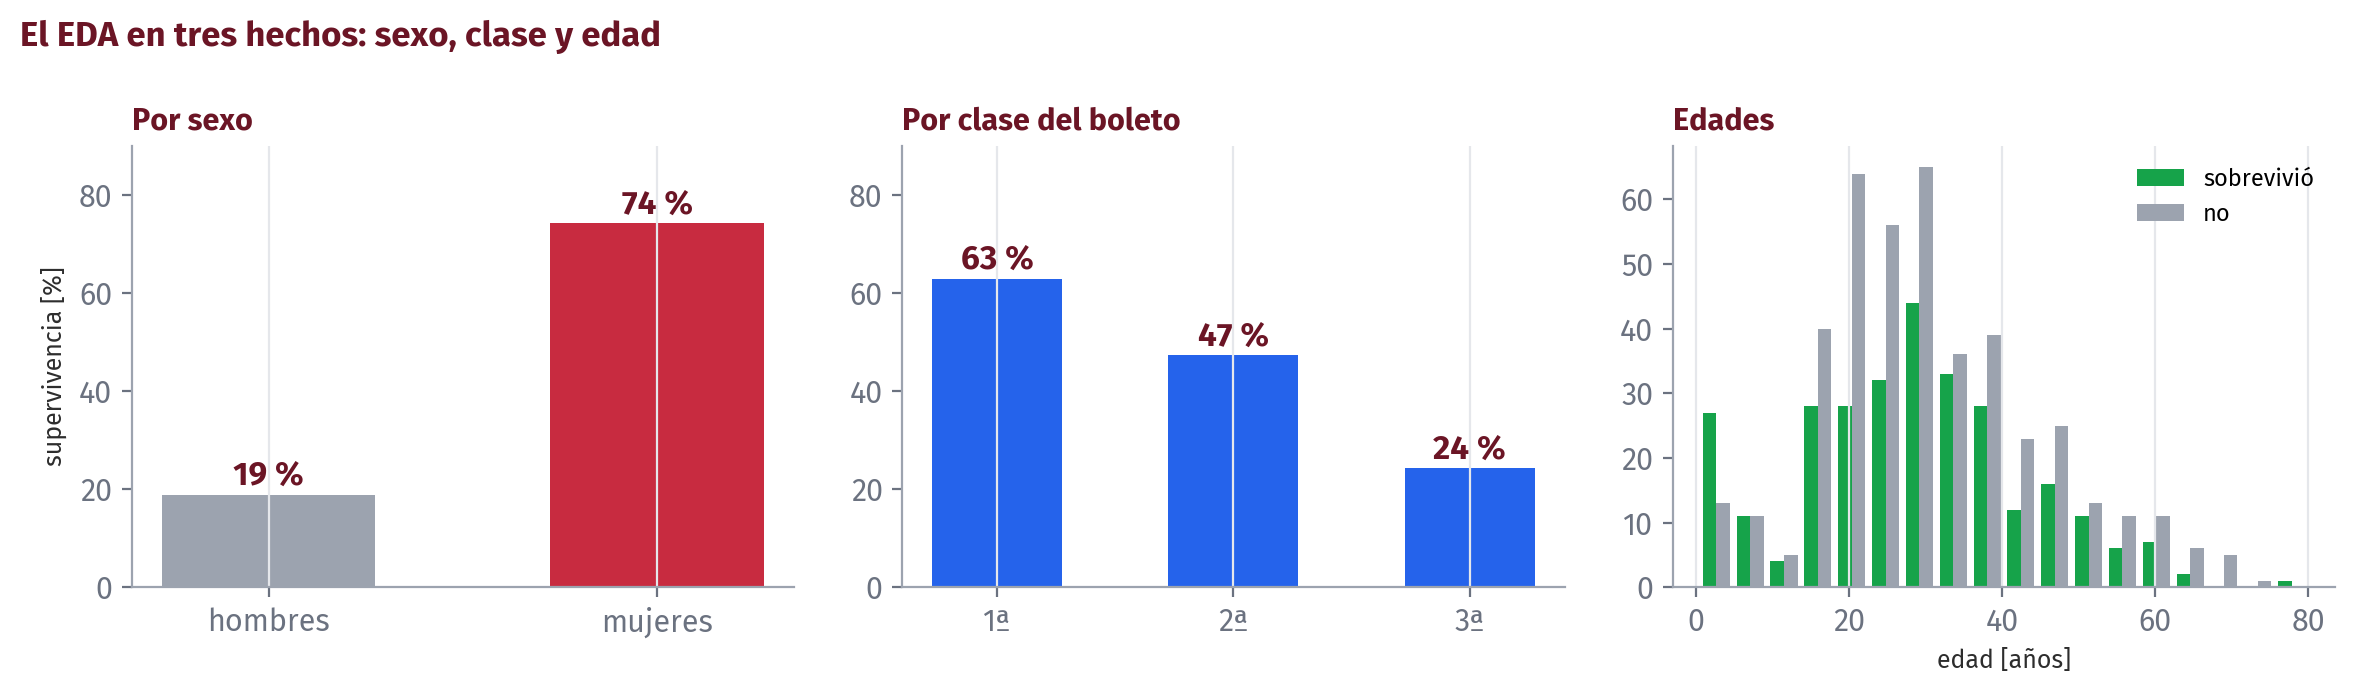
\includegraphics[width=0.96\textwidth, height=0.44\textheight, keepaspectratio]{fig_t_eda.png}\end{center}
  \vspace{2pt}
  {\footnotesize\color{textMuted}
   Tres hechos saltan solos: las mujeres sobrevivieron al \textbf{74\,\%} y
   los hombres al \textbf{19\,\%} («mujeres y niños primero»), la clase del
   boleto escalona todo, y entre los niños se sobrevivió más. Faltantes:
   edad 177, cubierta 688.}
\end{frame}

\begin{frame}[shrink=5]{La Trampa: el Modelo Perfecto que No Sirve}
  \vspace{2pt}
  {\scriptsize\color{textMuted}
   Entre las columnas sospechosas, el agente señaló \texttt{alive}: dice
   \texttt{yes}/\texttt{no}... y es \textbf{exactamente} \texttt{survived}
   disfrazado. ¿Qué pasa si se lo damos al modelo?}
  \vspace{2pt}
  \begin{tcolorbox}[colback=arcaGray, colframe=arcaRed, boxrule=0pt,
    leftrule=4pt, arc=3pt, left=10pt, right=10pt, top=4pt, bottom=4pt]
    \begin{center}
    {\Huge\color{arcaRed}\bfseries accuracy = 1.000}\\[2pt]
    {\scriptsize\color{textMuted}
     Tres líneas de código, cero errores... y cero utilidad: para saber
     \texttt{alive} hay que saber ya si sobrevivió.}
    \end{center}
  \end{tcolorbox}
  \vspace{2pt}
  {\scriptsize\color{textMuted}
   Esto se llama \textbf{fuga de información} (\emph{leakage}) y es el error
   más caro del ML en producción: el modelo brilla en el cuaderno y muere en
   el mundo real, donde la respuesta no viene incluida en los datos.}
  \vspace{2pt}
  {\scriptsize\color{arcaDark}\bfseries
   La regla que se llevan: si un modelo acierta casi todo, no celebren ---
   desconfíen. Lo perfecto huele a trampa.}
\end{frame}

\begin{frame}[shrink=5]{Paso 1 · Las Decisiones de Limpieza, Escritas}
  \vspace{2pt}
  {\footnotesize\color{textMuted}
  \begin{enumerate}\setlength{\itemsep}{5pt}
    \item \textbf{Fuera las columnas que repiten o derivan:} \texttt{alive}
          (la fuga), \texttt{class} y \texttt{embark\_town} (duplican en
          texto), \texttt{who}, \texttt{adult\_male}, \texttt{alone}
          (derivadas de sexo/edad/familia).
    \item \textbf{Fuera \texttt{deck}}: 688 de 891 faltantes (77\,\%) ---
          no hay con qué rellenar eso honestamente.
    \item \textbf{Edad}: 177 faltantes $\to$ la mediana. Es una decisión
          discutible, y por eso se \emph{escribe}.
    \item \textbf{Puerto}: 2 faltantes $\to$ el más común.
  \end{enumerate}}
  \vspace{6pt}
  \begin{tcolorbox}[colback=arcaGray, colframe=codeGreen, boxrule=0pt,
    leftrule=3pt, arc=3pt, left=9pt, right=9pt, top=5pt, bottom=5pt]
    {\footnotesize\color{arcaDark}\bfseries
     Quedan 7 columnas honestas: clase, sexo, edad, familia a bordo (2),
     tarifa y puerto. Con eso se compite.}
  \end{tcolorbox}
\end{frame}

\begin{frame}[shrink=5]{Paso 2 · GridSearch, Desde Cero}
  \vspace{2pt}
  {\footnotesize\color{textMuted
   }Hasta hoy siempre usamos \emph{un} modelo con \emph{una} receta. El flujo
   profesional prueba \textbf{varios modelos con varias recetas} y deja que
   los datos decidan. La herramienta se llama \texttt{GridSearchCV}, y el
   nombre se lee por partes:}
  \vspace{6pt}
  {\footnotesize\color{textMuted}
  \begin{itemize}\setlength{\itemsep}{5pt}
    \item[{\color{arcaRed}\scriptsize\faTh}]
      \textbf{Grid} --- la parrilla: todas las combinaciones de
      hiperparámetros que uno declara (profundidades, tasas de aprendizaje...).
    \item[{\color{arcaRed}\scriptsize\faSearch}]
      \textbf{Search} --- las prueba todas, una por una.
    \item[{\color{arcaRed}\scriptsize\faSyncAlt}]
      \textbf{CV} --- \emph{cross-validation}: cada receta rinde
      \textbf{cinco exámenes} con cinco particiones distintas del
      entrenamiento, y se promedia. Así una partición con suerte no corona a
      la receta equivocada.
  \end{itemize}}
  \vspace{6pt}
  {\footnotesize\color{arcaDark}\bfseries
   Y la regla de siempre, elevada al cuadrado: el examen final del 20\,\% se
   aparta ANTES --- ninguna búsqueda puede tocarlo. Se usa una sola vez, con
   el ganador.}
\end{frame}

\begin{frame}[shrink=5]{Paso 2 · El Encargo de la Comparación}
  \vspace{2pt}
  \begin{prompt}[EL PROMPT DE LA DEMO --- que decidan los datos]
Con el DataFrame `t` limpio (891 filas):

OBJETIVO: comparar tres modelos para predecir
survived, con búsqueda de hiperparámetros, y elegir
el mejor con honestidad.

RESTRICCIONES:
- candidatos: LogisticRegression (con StandardScaler
  en Pipeline), RandomForestClassifier y
  HistGradientBoostingClassifier
- GridSearchCV con cv=5 y accuracy, random_state=0
- reserva ANTES un 20% de examen final,
  estratificado, que ninguna búsqueda puede tocar
- categóricas con get_dummies

CRITERIO DE ACEPTACIÓN:
- una tabla: modelo, mejor receta, accuracy de
  validación cruzada
- el examen final se corre UNA sola vez, con el
  ganador
  \end{prompt}
\end{frame}

\begin{frame}[shrink=8]{Paso 2 · El Resultado de la Búsqueda}
  \vspace{-2pt}
  \begin{center}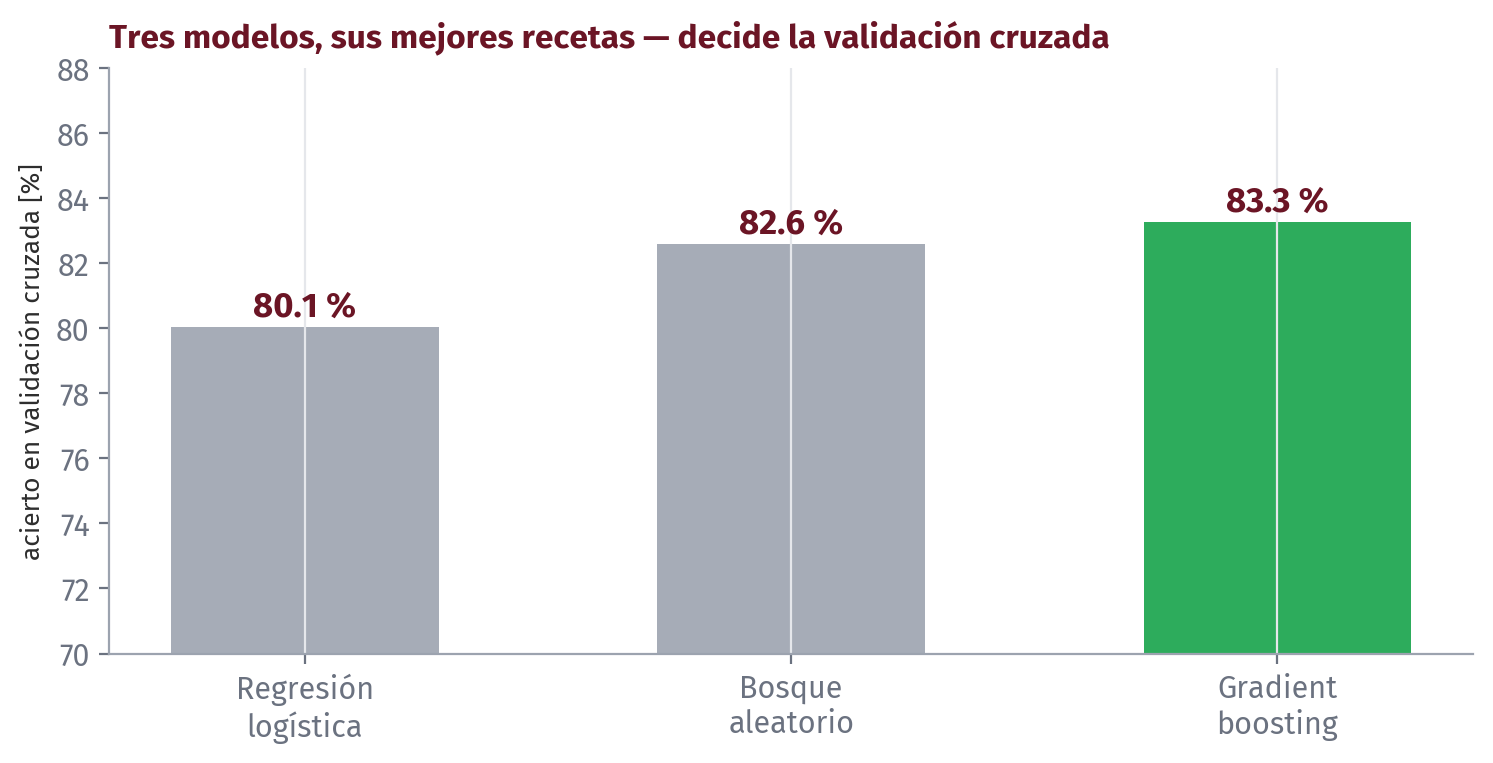
\includegraphics[width=0.80\textwidth, height=0.44\textheight, keepaspectratio]{fig_t_grid.png}\end{center}
  \vspace{2pt}
  {\footnotesize\color{textMuted}
   Los tres en un pañuelo --- 80,1 / 82,6 / 83,3 --- y gana el
   \textbf{gradient boosting}: árboles en cadena, cada uno aprende de los
   errores del anterior (primo del bosque, que vota en paralelo). Y noten lo
   que NO pasó: \textbf{nadie sacó 0.99} --- después de la fuga, un número
   así nos pararía en seco.}
\end{frame}

\begin{frame}[shrink=8]{Paso 3 · El Examen, en Probabilidades}
  \vspace{-2pt}
  \begin{center}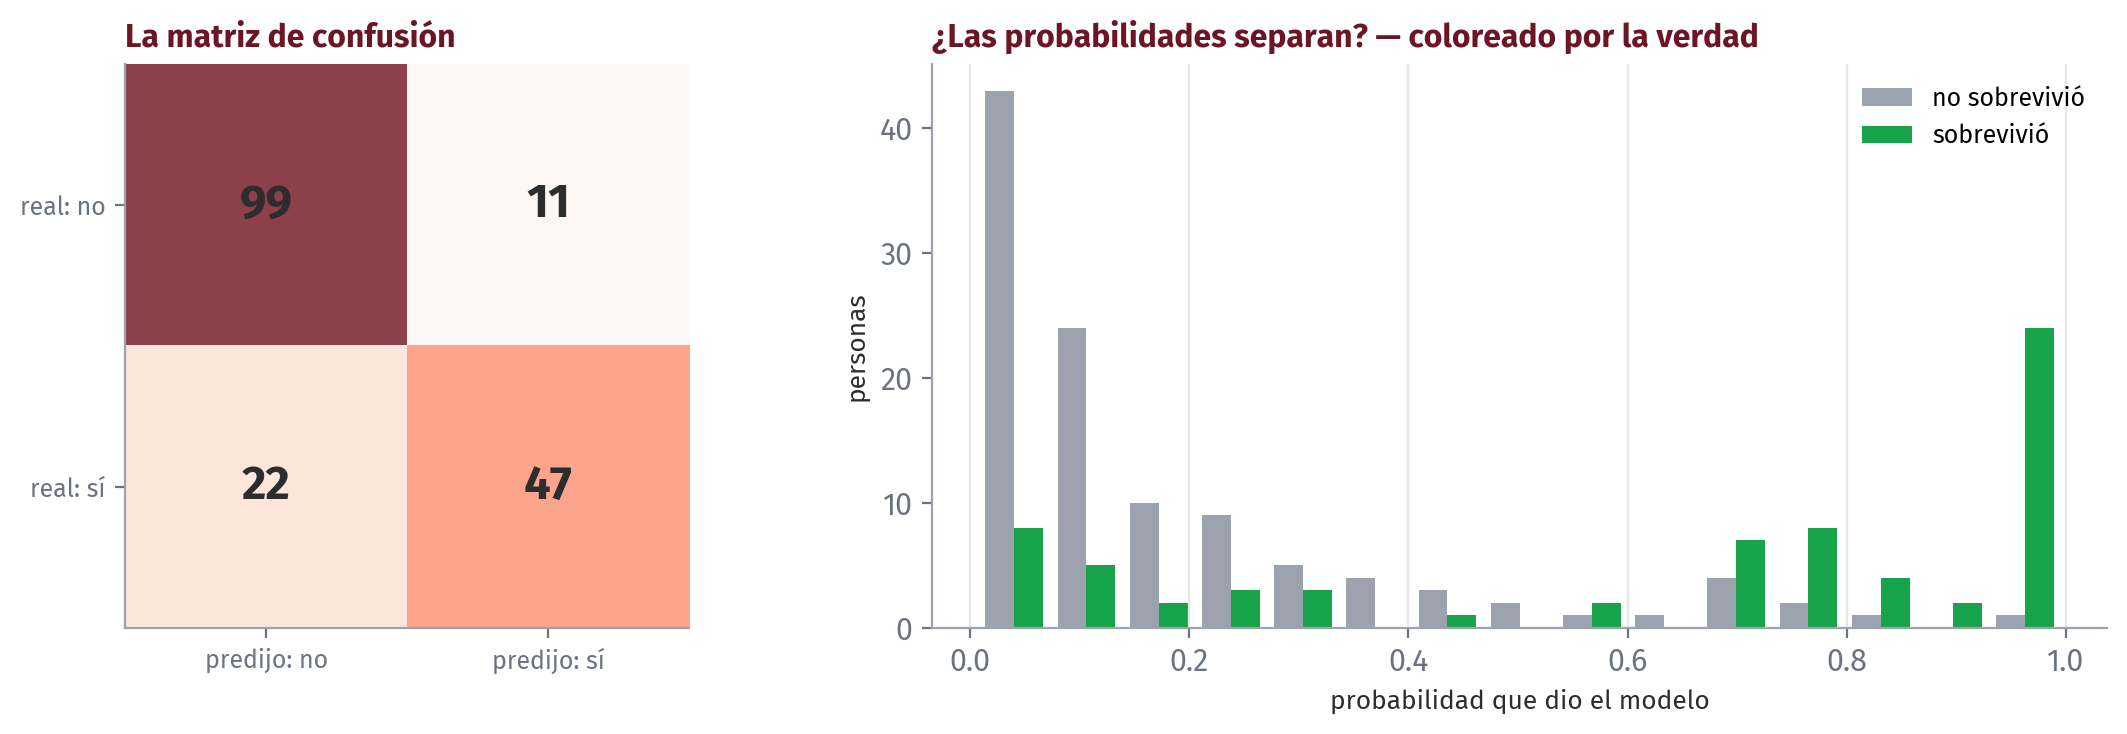
\includegraphics[width=0.97\textwidth, height=0.42\textheight, keepaspectratio]{fig_t_examen.png}\end{center}
  \vspace{2pt}
  {\footnotesize\color{textMuted}
   Examen final: \textbf{0.816} (146 de 179). Pero la salida honesta no es
   «sí/no»: es la \textbf{probabilidad} --- y la derecha muestra que valen:
   a las \textbf{32} personas a las que dio más de 80\,\%, sobrevivieron
   \textbf{30} (94\,\%).}
\end{frame}

\begin{frame}[shrink=5]{Paso 4 · Explicabilidad: SHAP, Desde Cero}
  \vspace{2pt}
  {\scriptsize\color{textMuted}
   Un 0.91 sin explicación no se puede defender en una reunión. La pregunta
   que siempre sigue al número es \emph{¿por qué?} --- y responderla tiene
   nombre: \textbf{SHAP}.}
  \vspace{2pt}
  \begin{tcolorbox}[colback=arcaGray, colframe=arcaDark, boxrule=0pt,
    leftrule=4pt, arc=3pt, left=10pt, right=10pt, top=4pt, bottom=4pt]
    {\scriptsize\color{arcaDark}\bfseries
     La idea, sin matemática: a cada variable se le asigna la parte
     \emph{justa} del empujón que dio --- cuánto movió la predicción hacia
     arriba o hacia abajo respecto del pasajero promedio.}\\[2pt]
    {\scriptsize\color{textMuted}
     Viene de la teoría de juegos (valores de \emph{Shapley}, premio Nobel
     2012 de por medio): cómo repartir el premio de un equipo entre sus
     jugadores según lo que aportó cada uno. Acá el «equipo» son las
     variables, y el «premio» es la predicción.}
  \end{tcolorbox}
  \vspace{2pt}
  {\scriptsize\color{textMuted}
   Dos niveles, y usamos ambos: \textbf{global} (qué manda en el modelo
   entero) e \textbf{individual} (los porqués de UNA predicción --- lo que la
   app le va a mostrar al usuario).}
\end{frame}

\begin{frame}[shrink=8]{Paso 4 · Qué Mueve la Predicción}
  \vspace{-2pt}
  \begin{center}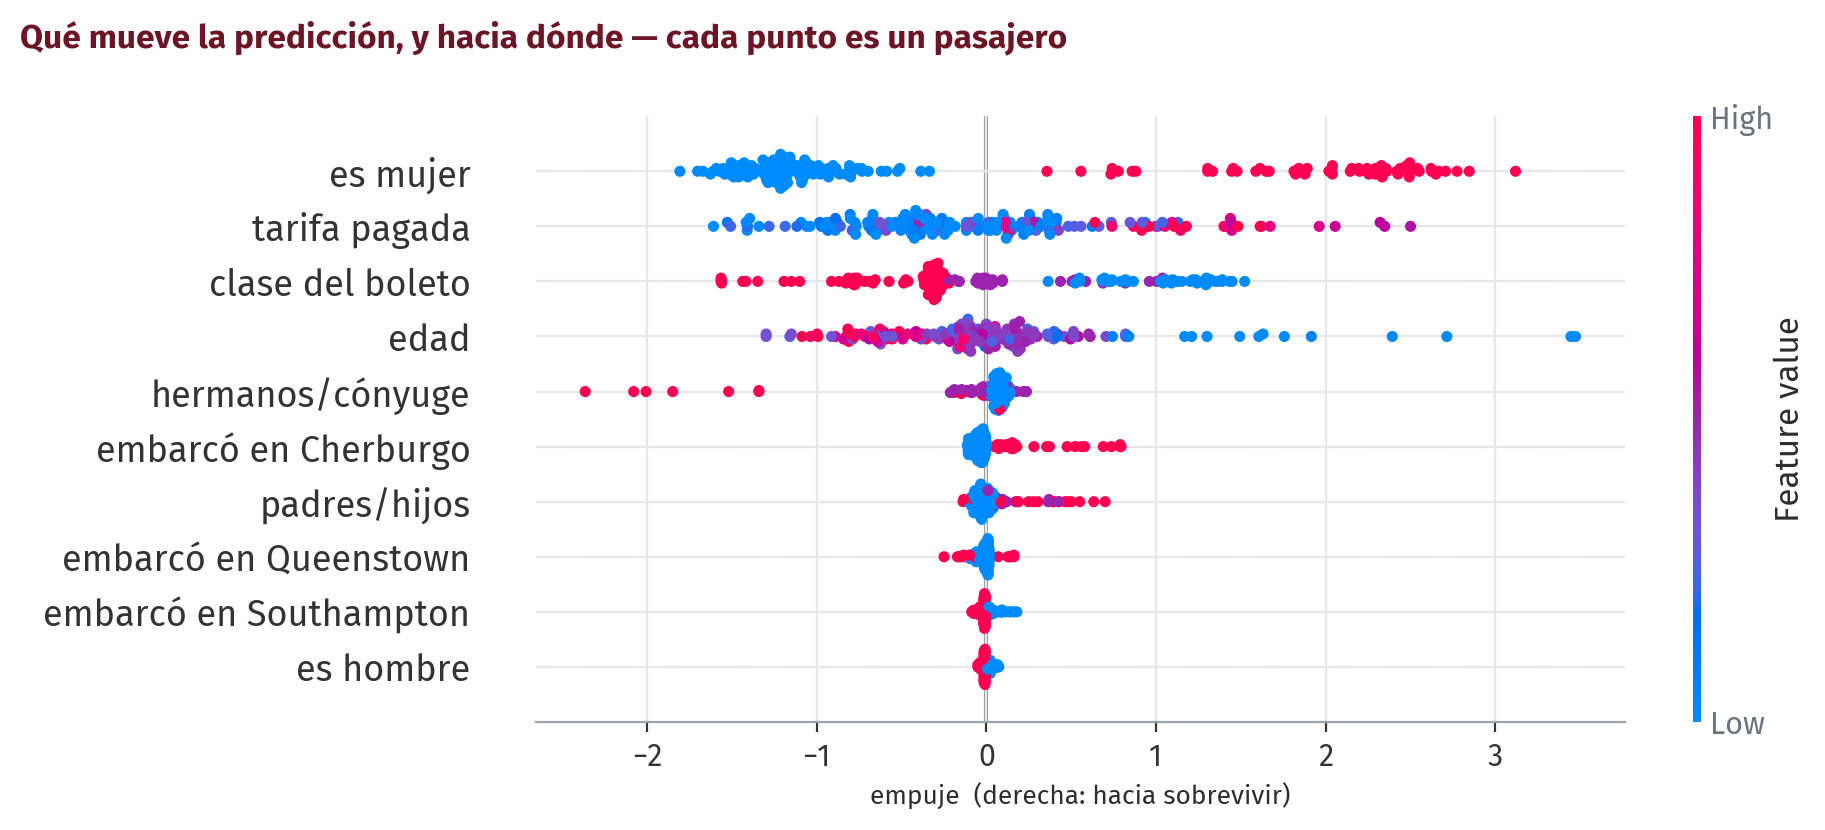
\includegraphics[width=0.86\textwidth, height=0.46\textheight, keepaspectratio]{fig_t_shap.png}\end{center}
  \vspace{2pt}
  {\scriptsize\color{textMuted}
   Cada punto es un pasajero; derecha = empuja a sobrevivir; el color es el
   valor (rojo alto). \textbf{Ser mujer/hombre parte el gráfico en dos};
   la 3ª clase (rojo en «clase») empuja a la izquierda; edad baja empuja a
   la derecha. \textbf{El modelo redescubrió, solo, el protocolo de
   evacuación de 1912.}}
\end{frame}

\begin{frame}[shrink=8]{Paso 4 · El Porqué de UNA Predicción}
  \vspace{-2pt}
  \begin{center}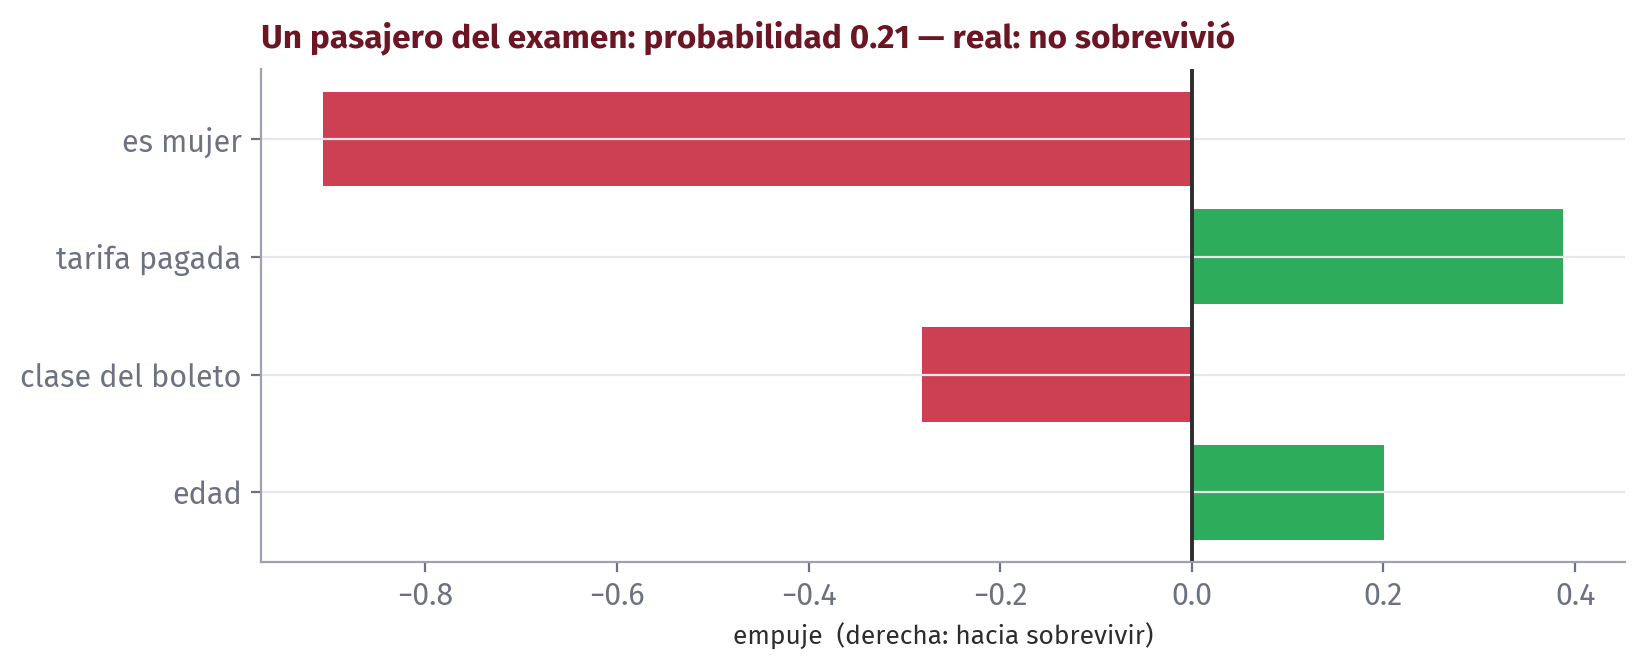
\includegraphics[width=0.86\textwidth, height=0.42\textheight, keepaspectratio]{fig_t_persona.png}\end{center}
  \vspace{2pt}
  {\footnotesize\color{textMuted}
   Un pasajero real del examen: probabilidad \textbf{0.21}, y sus cuatro
   factores con signo. Esto es lo que convierte un número en un argumento
   --- y es exactamente lo que la app entrega con cada predicción.}
\end{frame}

% ── GRADIO (reciclado de la version anterior de la clase) ────────────────────
\begin{frame}[shrink=8]{Gradio: Qué Es, y Por Qué Existe}
  \vspace{-6pt}
  \begin{columns}[T]
    \begin{column}{0.30\textwidth}
      \begin{center}
        
\includegraphics[width=0.52\linewidth]{_logos/gradio.png}\\[5pt]
        {\scriptsize\color{textMuted} desde 2021, parte de}\\[2pt]
        
\includegraphics[width=0.32\linewidth]{_logos/huggingface.png}\\[1pt]
        {\scriptsize\color{textMuted} Hugging Face}
      \end{center}
    \end{column}
    \begin{column}{0.66\textwidth}
      {\scriptsize\color{textMuted}
       Nació en \textbf{Stanford, en 2019}, por una frustración que les va a
       sonar: los investigadores tenían modelos médicos funcionando... y los
       \textbf{médicos} --- los que sabían si el modelo servía --- no podían
       probarlos sin pedirle una interfaz a un programador.
       \vspace{4pt}

       La solución fue radical: que \textbf{una función de Python se vuelva
       una página web} con controles, en una línea. Sin saber nada de
       páginas web.
       \vspace{4pt}

       Hoy es el \textbf{estándar de la industria} para poner un modelo en
       manos de alguien, y ya viene instalado en Colab.
       \vspace{4pt}

       \textbf{\color{arcaDark}Fíjense para quién se inventó: para que el
       experto de dominio tocara el modelo sin programar la interfaz. O sea:
       para ustedes.}}
    \end{column}
  \end{columns}
\end{frame}

\begin{frame}[fragile, shrink=5]{Gradio en Dos Escalones --- y el Link}
  \vspace{-2pt}
  {\scriptsize\color{textMuted}
   La anatomía completa en dos ejemplos de un minuto. \textbf{Escalón 1}:
   toda app son tres piezas --- función, entradas, salidas:}
  \vspace{2pt}
  \begin{minted}[fontsize=\scriptsize, breaklines]{python}
def saludar(nombre):
    return f"Hola, {nombre}"

gr.Interface(fn=saludar, inputs="text", outputs="text").launch()
  \end{minted}
  \vspace{2pt}
  {\scriptsize\color{textMuted}
   \textbf{Escalón 2}: controles con tipo, y \texttt{share=True} para el
   \textbf{link público} --- la dirección que otro abre desde su celular
   mientras su cuaderno trabaja por detrás:}
  \vspace{2pt}
  \begin{minted}[fontsize=\scriptsize, breaklines]{python}
gr.Interface(fn=a_metros_cubicos,
             inputs=gr.Number(label="Barriles [bbl]", value=1000),
             outputs=gr.Textbox(label="Metros cúbicos")
             ).launch(share=True)
  \end{minted}
  \vspace{2pt}
  {\scriptsize\color{arcaRed}\bfseries
   El link vive mientras el cuaderno corra.} {\scriptsize\color{textMuted}
   Perfecto para una demo o una jornada; no es un sistema permanente.}
\end{frame}

\begin{frame}[shrink=5]{Pasos 5 y 6 · La App, con Explicación y Contrato}
  \vspace{2pt}
  \begin{prompt}[EL PROMPT DE LA DEMO --- servir y blindar de una vez]
CONTEXTO: tengo `modelo` (el ganador), `explicador`
(shap.TreeExplainer), `columnas` (el orden del
entrenamiento) y el DataFrame limpio `t`.

OBJETIVO: app de Gradio --- perfil del pasajero
(clase, sexo, edad, hermanos/cónyuge, padres/hijos,
tarifa, puerto) y devuelve:
1. "X de cada 100 personas con este perfil
   sobrevivieron"
2. una gráfica con los 4 factores que más empujaron
   ESTA predicción

RESTRICCIONES:
- controles en español; rangos de edad y tarifa
  DESDE el dato `t`
- la fila para el modelo se arma como TABLA con las
  columnas en el orden de `columnas` (nunca números
  pelados)
- launch(share=True)

CRITERIO: una edad fuera del rango del dato se
rechaza con mensaje.
  \end{prompt}
  \vspace{3pt}
  {\scriptsize\color{arcaDark}\bfseries\itshape
   Probado en vivo: edad 500 $\to$ rechazada con mensaje. El contrato de
   entrada, la fila como tabla con nombres, la explicación en la salida ---
   todo lo de la clase pasada, junto.}
\end{frame}

% ═════════════════════════════════════════════════════════════════════════════
\sectionframe{Acto 2 · La Red que Ve}{Guiado: ustedes dirigen, el agente escribe \\[6pt] \normalsize 55 -- 115 min}
% ═════════════════════════════════════════════════════════════════════════════

\begin{frame}[shrink=5]{Cómo se Trabaja Este Acto}
  \vspace{-2pt}
  \begin{columns}[T]
    \begin{column}{0.62\textwidth}
      {\footnotesize\color{textMuted}
       Cuaderno nuevo: \textbf{La Red que Ve}. Guiado como la Clase 1:
      \begin{itemize}\setlength{\itemsep}{4pt}
        \item[{\color{codeGreen}\scriptsize\faCheck}]
          la \textbf{carga del dato viene dada} --- esa celda solo se corre
        \item[{\color{codeGreen}\scriptsize\faCheck}]
          cada paso trae su \textbf{prompt} listo para pegarle a Gemini
        \item[{\color{codeGreen}\scriptsize\faCheck}]
          la \textbf{tarea y el criterio} están escritos --- contra eso se
          revisa lo que devuelva
        \item[{\color{arcaRed}\scriptsize\faTimes}]
          soluciones escritas: \textbf{no hay}. Se construye acá.
      \end{itemize}}
      \vspace{4pt}
      {\scriptsize\color{arcaDark}\itshape
       Las herramientas nuevas del acto: \textbf{Keras} (la puerta de
       entrada a las redes, del equipo de Google) y \textbf{Ultralytics
       YOLO} (detección de objetos). Ambas gratis; Keras ya está en Colab.}
    \end{column}
    \begin{column}{0.32\textwidth}
      \begin{center}
        \vspace{2pt}
        
\includegraphics[width=0.44\linewidth]{_logos/keras.png}\\[2pt]
        {\scriptsize\color{textMuted} Keras}\\[8pt]
        
\includegraphics[width=0.44\linewidth]{_logos/ultralytics.png}\\[2pt]
        {\scriptsize\color{textMuted} Ultralytics YOLO}
      \end{center}
    \end{column}
  \end{columns}
\end{frame}

\begin{frame}[shrink=14]{El Puente: ¿Una Red le Ganaría al Boosting?}
  \vspace{2pt}
  {\scriptsize\color{textMuted}
   Si las redes son «lo más avanzado», ¿por qué no usamos una en el Titanic?
   Respuesta corta: \textbf{midámoslo}. El cuaderno les deja el récord a la
   vista:}
  \vspace{2pt}
  \begin{center}
  {\large\color{arcaDark}\bfseries EL RÉCORD A BATIR: 0.816}
  {\scriptsize\color{textMuted} --- el boosting, en el examen final}
  \end{center}
  \vspace{2pt}
  \begin{prompt}[SU PROMPT --- la red retadora]
CONTEXTO: tengo X_ent, X_exa, y_ent, y_exa (Titanic
limpio, examen del 20%, semilla 0). El récord a batir
es RECORD, de un gradient boosting.

OBJETIVO: una red en Keras para la misma tarea,
comparada contra el récord EN EL MISMO examen.

RESTRICCIONES: normaliza con StandardScaler (ajustado
solo con X_ent); dos capas relu y salida sigmoid;
early stopping; semillas fijas.

CRITERIO: los dos números lado a lado, y nada de
tocar X_exa hasta el final.
  \end{prompt}
  \vspace{2pt}
  {\scriptsize\color{arcaDark}\bfseries Antes de correr: apuesten. ¿Quién gana, y por cuánto?}
\end{frame}

\begin{frame}[shrink=5]{La Lección Honesta de 2026}
  \vspace{2pt}
  \begin{tcolorbox}[colback=arcaGray, colframe=arcaRed, boxrule=0pt,
    leftrule=4pt, arc=3pt, left=10pt, right=10pt, top=4pt, bottom=4pt]
    {\large\color{arcaDark}\bfseries
     En datos tabulares --- filas y columnas, como casi todo lo que ustedes
     manejan --- los árboles siguen mandando.}
  \end{tcolorbox}
  \vspace{2pt}
  {\scriptsize\color{textMuted}
   No es una opinión: es el resultado repetido de las competencias y los
   estudios comparativos de estos años, y lo acaban de medir ustedes mismos.
   ¿Por qué pasa?
  \begin{itemize}\setlength{\itemsep}{2pt}
    \item[{\color{arcaRed}\scriptsize\faArrowRight}]
      En una tabla, cada columna significa algo distinto (edad, tarifa,
      clase) --- no hay una \emph{estructura} que la red pueda explotar.
    \item[{\color{arcaRed}\scriptsize\faArrowRight}]
      Los árboles cortan por umbrales («edad $<$ 12») --- que es exactamente
      la forma de las reglas del mundo tabular.
    \item[{\color{arcaRed}\scriptsize\faArrowRight}]
      Con cientos de filas, una red tiene poco de dónde aprender; el
      boosting exprime más lo poco.
  \end{itemize}}
  \vspace{2pt}
  {\scriptsize\color{arcaDark}\bfseries
   Las redes brillan donde NO hay tabla: imágenes, señales, texto ---
   donde la estructura lo es todo. Vamos allá.}
\end{frame}

\begin{frame}[shrink=5]{La No Linealidad: la Pregunta}
  \vspace{2pt}
  {\footnotesize\color{textMuted}
   Antes de las imágenes, el concepto que hace distintas a las redes ---
   \textbf{visto}, no contado. El cuaderno les genera 250 puntos en dos
   medias lunas entrelazadas, y la pregunta es: ¿puede una línea recta
   separarlas?}
  \vspace{5pt}
  \begin{prompt}[SU PROMPT --- las dos fronteras]
CONTEXTO: tengo `puntos` (250 filas, 2 columnas) y
`etiqueta` (0/1) de make_moons: dos medias lunas
entrelazadas.

OBJETIVO: mostrar visualmente qué puede y qué no
puede cada modelo.
- entrena una LogisticRegression y un MLPClassifier
  (hidden_layer_sizes=(16, 16), max_iter=3000,
  random_state=0)
- dibuja las dos FRONTERAS DE DECISIÓN lado a lado,
  con los puntos encima, títulos en español, y el
  acierto de cada uno en el título

CRITERIO: que se VEA de un vistazo cuál de los dos
puede curvar la frontera.
  \end{prompt}
  \vspace{3pt}
  {\scriptsize\color{arcaDark}\itshape
   Tarea: cuando salga, una frase por pregunta --- ¿por qué la recta no
   puede? ¿qué le permite a la red curvarse?}
\end{frame}

\begin{frame}[shrink=8]{La No Linealidad: la Respuesta, Leída Juntos}
  \vspace{-2pt}
  \begin{center}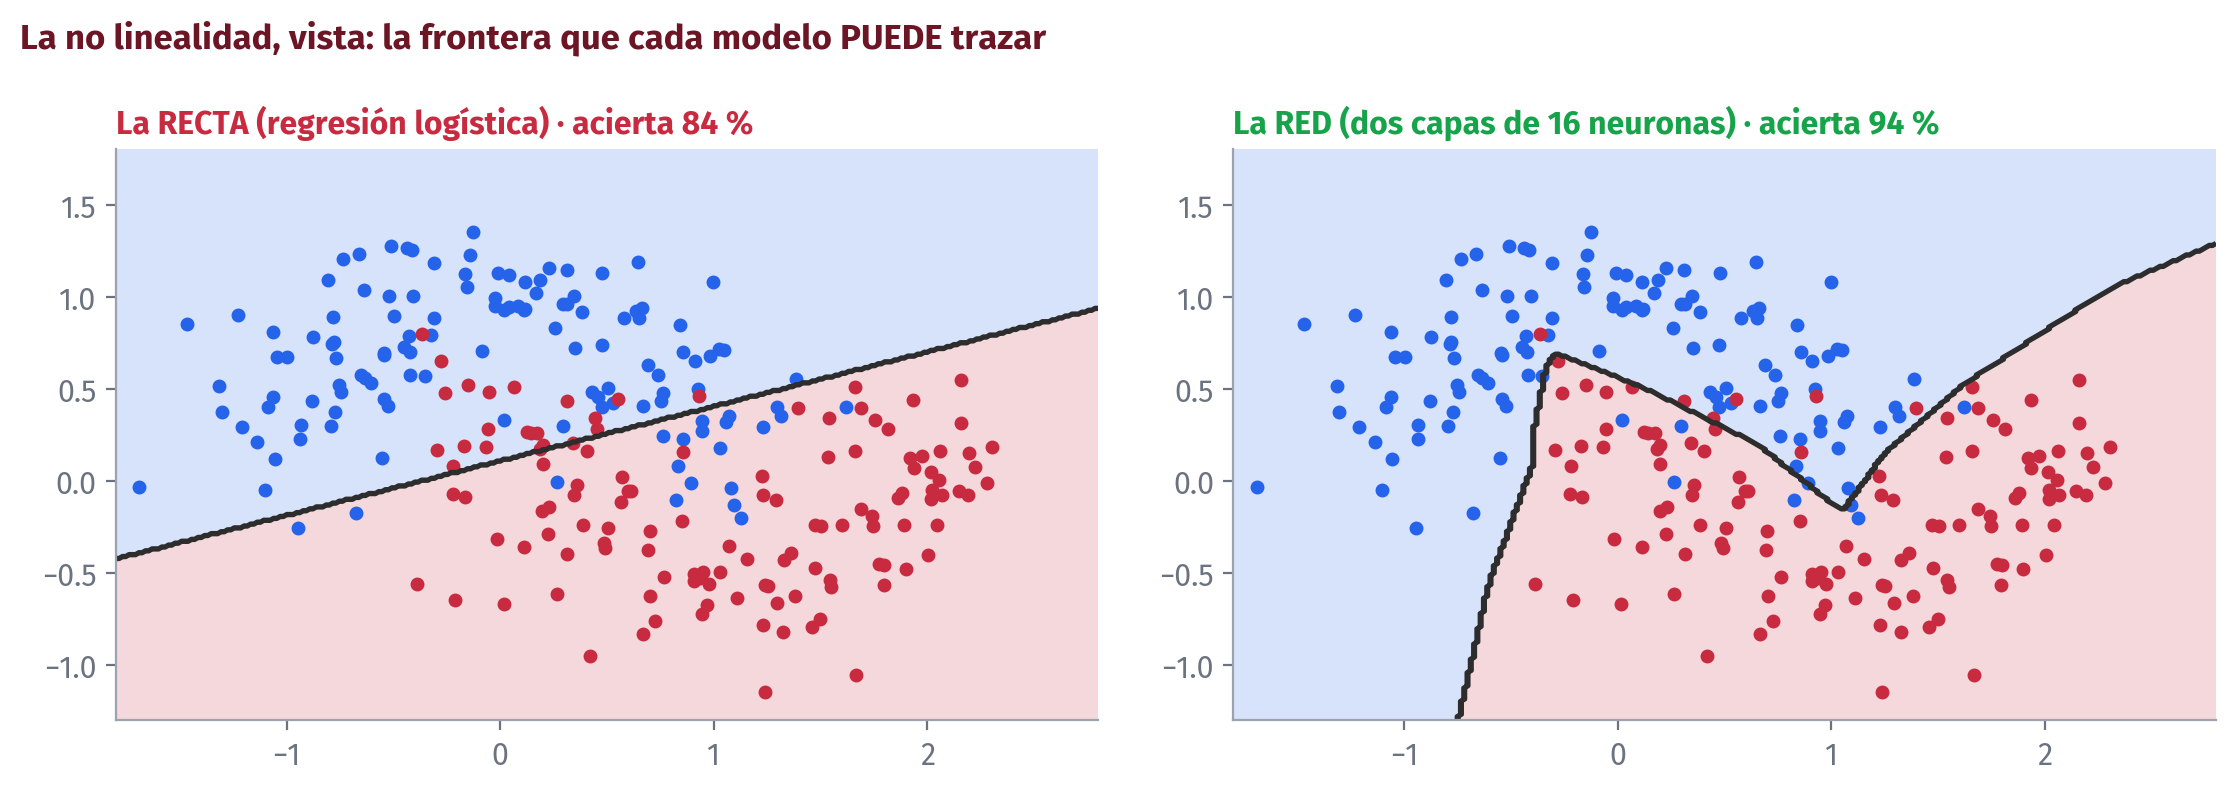
\includegraphics[width=0.94\textwidth, height=0.44\textheight, keepaspectratio]{fig_moons.png}\end{center}
  \vspace{2pt}
  {\footnotesize\color{textMuted}
   La recta acierta \textbf{84\,\%} --- su mejor recta posible. La red,
   \textbf{94\,\%}, porque puede \textbf{curvar}. El secreto completo: cada
   neurona es \emph{suma ponderada + un doblez} (la activación); apilar
   capas de dobleces permite \textbf{componer curvas}. Eso es una red
   neuronal.}
\end{frame}

\begin{frame}[shrink=8]{MNIST: Donde No Hay Tabla}
  \vspace{-2pt}
  \begin{center}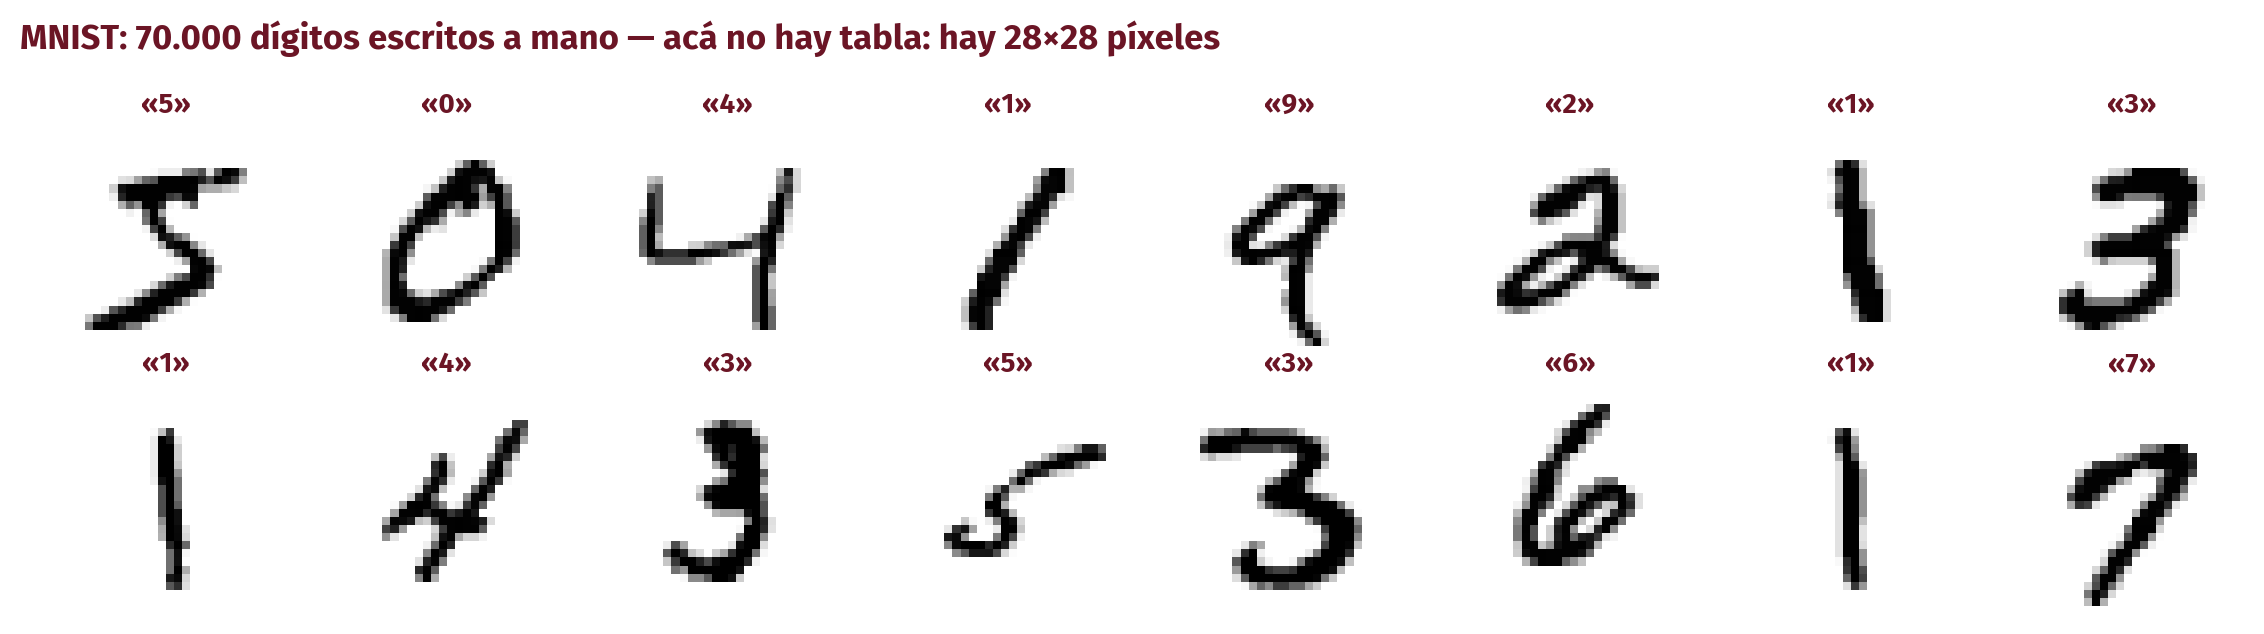
\includegraphics[width=0.92\textwidth, height=0.40\textheight, keepaspectratio]{fig_mnist.png}\end{center}
  \vspace{2pt}
  {\footnotesize\color{textMuted}
   El «hola mundo» de las redes desde hace treinta años: \textbf{70.000
   dígitos} escritos a mano, cada uno una imagen de 28×28. Aquí no hay
   columnas con significado: hay \textbf{784 píxeles con estructura} --- el
   terreno de la red. Y los píxeles van de 0 a 255: ahí entra la
   \textbf{normalización} (todo a 0--1, dividiendo por 255).}
\end{frame}

\begin{frame}[shrink=5]{Su Primera Red que Lee}
  \vspace{2pt}
  \begin{prompt}[SU PROMPT --- armar y entrenar]
CONTEXTO: tengo x_ent, y_ent, x_exa, y_exa de
keras.datasets.mnist. Imágenes de 28x28 con píxeles
0-255; etiquetas 0-9.

OBJETIVO: mi primera red neuronal en Keras que
clasifique los dígitos.

RESTRICCIONES:
- normaliza dividiendo por 255, y aplana cada imagen
  a 784 valores
- red simple: Dense(128, relu) -> Dense(10, softmax)
- compila con adam y sparse_categorical_crossentropy
- entrena 8 épocas con validation_split=0.1
- guarda el history en una variable

CRITERIO DE ACEPTACIÓN:
- más de 97% de acierto en validación
- el examen con x_exa se corre UNA sola vez, al final
  \end{prompt}
  \vspace{3pt}
  {\scriptsize\color{arcaDark}\bfseries\itshape
   Mientras entrena, miren la barra época por época: están viendo a la red
   aprender. Ocho épocas, un par de minutos, más del 97 \%.}
\end{frame}

\begin{frame}[shrink=5]{El Overfitting, Visto en Vivo}
  \vspace{-2pt}
  \begin{columns}[T]
    \begin{column}{0.40\textwidth}
      \vspace{6pt}
      \begin{center}
      \begin{tikzpicture}[scale=0.82]
        \draw[-{Stealth}, color=gray] (0,0) -- (4.6,0)
          node[below, font=\tiny, text=textMuted] {épocas};
        \draw[-{Stealth}, color=gray] (0,0) -- (0,3.1)
          node[left, font=\tiny, text=textMuted, rotate=90, anchor=south] {acierto};
        \draw[line width=1.6pt, color=arcaDark]
          (0.2,0.6) .. controls (1.4,2.2) and (2.6,2.6) .. (4.3,2.9);
        \draw[line width=1.6pt, color=arcaRed, dashed]
          (0.2,0.55) .. controls (1.4,2.0) and (2.4,2.3) .. (3.0,2.35)
          .. controls (3.6,2.38) and (4.0,2.3) .. (4.3,2.2);
        \draw[color=gray, dotted, line width=1pt] (2.9,0) -- (2.9,2.5);
        \node[font=\tiny, text=arcaRed, align=center] at (3.5,1.2)
          {aquí empieza\\a memorizar};
        \node[font=\tiny, text=arcaDark] at (1.5,2.75) {entrenamiento};
        \node[font=\tiny, text=arcaRed] at (1.6,1.35) {validación};
      \end{tikzpicture}
      \end{center}
      {\scriptsize\color{textMuted}\itshape\centering
       El esquema. El real lo dibujan ustedes ahora.\par}
    \end{column}
    \begin{column}{0.56\textwidth}
      \begin{prompt}[SU PROMPT --- las curvas]
Con el `history` del entrenamiento:
grafica accuracy y loss de entrenamiento
y de validación por época, lado a lado,
en español. Marca la zona donde el
entrenamiento sigue mejorando pero la
validación ya no.
      \end{prompt}
      \vspace{3pt}
      {\scriptsize\color{textMuted}
       \textbf{Tarea:} ¿en qué época se separan sus curvas? Esa separación
       \textbf{es} el overfitting: la red memorizando en vez de aprender.\\[3pt]
       \textbf{La medicina} se llama regularización: parar antes
       (\emph{early stopping}) o penalizar la complejidad.}
    \end{column}
  \end{columns}
\end{frame}

\begin{frame}[shrink=5]{La Parte Honesta: ¿En Qué Se Equivoca?}
  \vspace{2pt}
  \begin{prompt}[SU PROMPT --- los errores, con la cara del modelo]
Con la red entrenada y el examen x_exa:
- la matriz de confusión 10x10
- muéstrame 9 dígitos donde la red se equivocó, con
  lo que ella creyó, su confianza, y la etiqueta real
  \end{prompt}
  \vspace{6pt}
  {\footnotesize\color{textMuted}
   \textbf{Tarea:} miren sus nueve errores y respondan:
  \begin{itemize}\setlength{\itemsep}{4pt}
    \item[{\color{arcaRed}\scriptsize\faQuestion}]
      ¿Qué pares se confunden --- ¿el 4 con el 9? ¿el 3 con el 5?
    \item[{\color{arcaRed}\scriptsize\faQuestion}]
      ¿Los errores son \emph{razonables} --- se equivocaría también un humano
      con esa caligrafía?
    \item[{\color{arcaRed}\scriptsize\faQuestion}]
      ¿La confianza del modelo en sus errores es alta o baja? ¿Qué implicaría
      eso si esta red leyera cheques?
  \end{itemize}}
  \vspace{5pt}
  {\footnotesize\color{arcaDark}\bfseries\itshape
   Mirar los errores de un modelo a la cara es la costumbre que separa a
   quien lo usa de quien le cree.}
\end{frame}

\begin{frame}[shrink=5]{El Salto de 2026: No Entrenar --- Dirigir}
  \vspace{2pt}
  {\scriptsize\color{textMuted}
   Su red aprendió 10 dígitos con 60.000 ejemplos. Los modelos grandes de
   visión aprendieron \textbf{cientos de clases con millones de imágenes} ---
   y ya están entrenados, gratis, a un \texttt{pip install} de distancia.}
  \vspace{2pt}
  \begin{tcolorbox}[colback=arcaGray, colframe=arcaDark, boxrule=0pt,
    leftrule=4pt, arc=3pt, left=10pt, right=10pt, top=4pt, bottom=4pt]
    {\scriptsize\color{arcaDark}\bfseries
     YOLO (\emph{You Only Look Once}): una red convolucional que detecta y
     ubica objetos en una imagen, en tiempo real.}\\[2pt]
    {\scriptsize\color{textMuted}
     «Convolucional»: en vez de mirar píxel por píxel, aprende
     \emph{patrones locales} (bordes, texturas, formas) y los compone ---
     la misma idea de apilar dobleces, llevada a imágenes.}
  \end{tcolorbox}
  \vspace{2pt}
  \begin{prompt}[SU PROMPT --- la primera detección]
OBJETIVO: probar un modelo YOLO preentrenado.
- carga el modelo "yolo11n.pt" con ultralytics
- detecta objetos en esta imagen de prueba:
  https://ultralytics.com/images/bus.jpg
- muestra la imagen con las cajas dibujadas, y debajo
  un conteo por tipo de objeto, en español
  \end{prompt}
\end{frame}

\begin{frame}[shrink=5]{Ahora con SUS Fotos --- y la App}
  \vspace{2pt}
  {\scriptsize\color{textMuted}
   Suban una foto del celular (panel \faFolder\ de Colab) y pásenla por el
   mismo detector.}
  \vspace{2pt}
  \begin{tcolorbox}[colback=arcaGray, colframe=arcaRed, boxrule=0pt,
    leftrule=3pt, arc=3pt, left=8pt, right=8pt, top=4pt, bottom=4pt]
    {\scriptsize\color{arcaRed}\bfseries ANTES DE SUBIR NADA}\\[2pt]
    {\scriptsize\color{textMuted}
     Nada de instalaciones de la empresa, documentos, ni personas sin
     permiso. La calle, su escritorio, el parqueadero. El porqué completo,
     en la Clase 4.}
  \end{tcolorbox}
  \vspace{2pt}
  \begin{prompt}[SU PROMPT --- la app que cierra el día]
OBJETIVO: una app de Gradio: el usuario sube una
imagen y recibe la imagen con las detecciones
dibujadas, más el conteo por tipo de objeto en
español.

RESTRICCIONES: gr.Image de entrada y salida,
launch(share=True); si no se detecta nada, decirlo
con un mensaje claro.

CRITERIO: que un compañero pueda usarla desde el
link, con su foto.
  \end{prompt}
\end{frame}

% ═════════════════════════════════════════════════════════════════════════════
\sectionframe{Cierre}{}
% ═════════════════════════════════════════════════════════════════════════════

\begin{frame}[shrink=5]{El Arco Completo, en Una Tabla}
  \vspace{6pt}
  \begin{center}
  {\footnotesize
  \begin{tabular}{lll}
    \toprule
    \textbf{El dato} & \textbf{Quién manda} & \textbf{Lo que hicieron hoy} \\
    \midrule
    Tablas (filas × columnas) & Los árboles: bosque, boosting &
    Titanic: GridSearch, SHAP, app \\[3pt]
    Imágenes, señales, texto & Las redes neuronales &
    MNIST: su primera red en Keras \\[3pt]
    Lo ya entrenado por otros & Ustedes, dirigiendo &
    YOLO: detectar sin entrenar \\
    \bottomrule
  \end{tabular}}
  \end{center}
  \vspace{9pt}
  {\footnotesize\color{textMuted}
   Y el mapeo a su mundo, dicho y no ejercitado: detección de EPP en cámaras
   de planta, lectura de medidores análogos, corrosión en fotos de
   inspección, conteo de inventario en patio. Todos son «YOLO con ajuste
   fino» --- un curso que ya están en condiciones de tomar.}
  \vspace{6pt}
  {\footnotesize\color{arcaDark}\bfseries\itshape
   La herramienta cambia con el dato. El método --- certificar, examinar,
   explicar, blindar --- no cambia nunca.}
\end{frame}

\begin{frame}[shrink=8]{Lo Que Aprendimos Hoy}
  \vspace{-2pt}
  \begin{columns}[T]
    \begin{column}{0.48\textwidth}
      {\small\color{arcaDark}\bfseries\faLightbulb[regular]\hspace{5pt}Conceptos:}
      \vspace{4pt}
      {\footnotesize\color{textMuted}
      \begin{itemize}\setlength{\itemsep}{3pt}
        \item[{\color{codeGreen}\scriptsize\faCheck}]
          La \textbf{fuga de información} --- lo perfecto huele a trampa
        \item[{\color{codeGreen}\scriptsize\faCheck}]
          \textbf{GridSearch + CV}: que decidan los datos, no el gusto
        \item[{\color{codeGreen}\scriptsize\faCheck}]
          \textbf{SHAP}: el porqué global y el de cada predicción
        \item[{\color{codeGreen}\scriptsize\faCheck}]
          La \textbf{no linealidad}: neurona = suma + doblez
        \item[{\color{codeGreen}\scriptsize\faCheck}]
          El \textbf{overfitting}, visto en sus propias curvas
      \end{itemize}}
    \end{column}
    \begin{column}{0.48\textwidth}
      {\small\color{arcaDark}\bfseries\faTools\hspace{5pt}Herramientas:}
      \vspace{4pt}
      {\footnotesize\color{textMuted}
      \begin{itemize}\setlength{\itemsep}{3pt}
        \item[{\color{arcaRed}\scriptsize\faArrowRight}]
          \texttt{GridSearchCV} y \texttt{predict\_proba}
        \item[{\color{arcaRed}\scriptsize\faArrowRight}]
          \texttt{shap} --- TreeExplainer
        \item[{\color{arcaRed}\scriptsize\faArrowRight}]
          \texttt{keras} --- Dense, relu, softmax, history
        \item[{\color{arcaRed}\scriptsize\faArrowRight}]
          \texttt{ultralytics} --- YOLO preentrenado
        \item[{\color{arcaRed}\scriptsize\faArrowRight}]
          \texttt{gradio} --- por fin, el link
      \end{itemize}}
      \vspace{5pt}
      \begin{tcolorbox}[colback=arcaGray, colframe=arcaRed, boxrule=0pt, leftrule=3pt,
        arc=3pt, left=6pt, right=6pt, top=4pt, bottom=4pt]
        {\scriptsize\color{arcaRed}\bfseries EL NÚMERO DEL DÍA}\\[3pt]
        {\scriptsize\color{textMuted}
         \textbf{1.000.} El accuracy del modelo con la columna tramposa.
         El número perfecto era el único imposible.}
      \end{tcolorbox}
    \end{column}
  \end{columns}
\end{frame}

\begin{frame}[shrink=5]{Los Resultados Negativos de Hoy}
  \vspace{2pt}
  {\scriptsize\color{textMuted}
   Como siempre, en voz alta:}
  \vspace{2pt}
  {\scriptsize\color{textMuted}
  \begin{enumerate}\setlength{\itemsep}{2pt}
    \item[{\color{arcaRed}\scriptsize\faTimes}]
      \textbf{La columna \texttt{alive} daba accuracy 1.000} --- y cero
      utilidad. La fuga de información no avisa: se busca.
    \item[{\color{arcaRed}\scriptsize\faTimes}]
      \textbf{La red neuronal no le ganó al boosting} en la tabla del
      Titanic. En tabular, los árboles mandan --- elegir por moda es caro.
    \item[{\color{arcaRed}\scriptsize\faTimes}]
      \textbf{Su propia red hizo overfitting} --- y lo vieron en sus curvas.
      Por eso el examen se reserva antes, siempre.
    \item[{\color{arcaRed}\scriptsize\faTimes}]
      \textbf{YOLO también falla} --- y lo anotaron. Preentrenado no es
      infalible: el trabajo se movió a dirigir y verificar.
  \end{enumerate}}
  \vspace{2pt}
  \begin{tcolorbox}[colback=arcaGray, colframe=arcaDark, boxrule=0pt,
    leftrule=4pt, arc=3pt, left=10pt, right=10pt, top=4pt, bottom=4pt]
    {\scriptsize\color{arcaDark}\bfseries
     Cuatro fallas medidas en una clase. Eso no es mala suerte: es lo que se
     ve cuando uno mira. Los que no las ven, las despliegan.}
  \end{tcolorbox}
\end{frame}

\begin{frame}[shrink=5]{Si Se Llevan Una Sola Cosa}
  \vspace{6pt}
  \begin{tcolorbox}[colback=arcaGray, colframe=arcaRed, boxrule=0pt, leftrule=4pt,
    arc=3pt, left=10pt, right=10pt, top=9pt, bottom=9pt]
    {\large\color{arcaDark}\bfseries
     La herramienta se elige midiendo, no por moda --- y el número perfecto
     es el único al que jamás hay que creerle.}\\[6pt]
    {\footnotesize\color{textMuted}
     Hoy compitieron cuatro modelos y una red. Ganó el que ganó \emph{en el
     examen}, no el más famoso. Y el único que sacó 100 era una trampa.\\[5pt]
     Ese par de reflejos --- medir antes de elegir, desconfiar de lo
     perfecto --- vale más que cualquier algoritmo de este curso.}
  \end{tcolorbox}
  \vspace{7pt}
  {\footnotesize\color{arcaDark}\itshape
   Y salieron sabiendo qué es una red neuronal, habiendo entrenado una, y
   habiendo dirigido a la más famosa del mundo. Nada mal para una tarde.}
\end{frame}

\begin{frame}[shrink=5]{Su Proyecto: la Plantilla Quedó Lista}
  \vspace{2pt}
  {\scriptsize\color{textMuted}
   El cuaderno del Titanic \textbf{es la plantilla de su entrega}. Con su
   dato, el flujo es idéntico:}
  \vspace{2pt}
  {\scriptsize\color{textMuted}
  \begin{enumerate}\setlength{\itemsep}{2pt}
    \item \textbf{EDA} --- y la pregunta por las columnas sospechosas
    \item \textbf{Limpieza} con decisiones escritas
    \item \textbf{Comparación de modelos} (GridSearch, cv=5)
    \item \textbf{Examen} reservado antes, corrido una vez
    \item \textbf{Explicabilidad} --- global y por predicción
    \item \textbf{La app} con link, contrato de entrada y explicación
  \end{enumerate}}
  \vspace{2pt}
  \begin{tcolorbox}[colback=arcaGray, colframe=codeGreen, boxrule=0pt, leftrule=3pt,
    arc=3pt, left=8pt, right=8pt, top=4pt, bottom=4pt]
    {\scriptsize\color{codeGreen}\bfseries\faCheck\hspace{4pt}LA ENTREGA}\\[3pt]
    {\scriptsize\color{textMuted}
     Hasta el \textbf{jueves de la próxima semana}, equipos de hasta 3: el
     cuaderno con el flujo completo, la app con link, los prompts que
     usaron, y \textbf{un error del agente que ustedes cazaron}. Si su dato
     es tabular --- casi seguro --- ya saben qué familia de modelos probar
     primero, y por qué.}
  \end{tcolorbox}
\end{frame}

\begin{frame}[shrink=8]{Datos y Referencias}
  \vspace{4pt}
  {\footnotesize\color{textMuted}
  \begin{itemize}\setlength{\itemsep}{5pt}
    \item[{\color{arcaRed}\scriptsize\faDatabase}]
      \textbf{Datos:} \texttt{pasajeros\_titanic} en el repositorio del
      curso (copia exacta del conjunto de práctica de seaborn);
      \textbf{MNIST} vía \texttt{keras.datasets}; imagen de prueba de
      Ultralytics.
    \item[{\color{arcaRed}\scriptsize\faBook}]
      \textbf{SHAP}: Lundberg \& Lee (2017), sobre los valores de Shapley
      (1953). \textbf{Keras}: equipo de Google. \textbf{YOLO}: Redmon et
      al.\ (2016); implementación moderna de Ultralytics.
    \item[{\color{arcaRed}\scriptsize\faFileCode}]
      Las cifras del Acto 1 salen de \texttt{figuras.py} y el cuaderno de
      la demo las reproduce exactamente. Del Acto 2 \textbf{no hay
      soluciones escritas}: se construye en clase dirigiendo al agente.
  \end{itemize}}
  \vspace{7pt}
  {\scriptsize\color{arcaDark}\itshape
   Como siempre: corren los scripts y tiene que dar exactamente lo mismo. Si
   no da, es un error nuestro y queremos saberlo.}
\end{frame}

% ── GRACIAS ──────────────────────────────────────────────────────────────────
\begingroup
\setbeamertemplate{headline}{}
\setbeamertemplate{footline}{}
\setbeamertemplate{navigation symbols}{}
\begin{frame}[plain, noframenumbering]
  \begin{tikzpicture}[remember picture, overlay]
    \fill[arcaDark] (current page.south west) rectangle (current page.north east);
    \node[anchor=center, text=white, font=\Huge\bfseries]
      at ([yshift=1.5cm]current page.center) {¡Gracias!};
    \node[anchor=center, text=white!80, font=\large, text width=10cm, align=center]
      at ([yshift=0.2cm]current page.center)
      {Carlos Enrique Mosquera Trujillo};
    \node[anchor=center, text=white!60, font=\normalsize, text width=10cm, align=center]
      at ([yshift=-0.6cm]current page.center)
      {\faEnvelope\hspace{6pt}cmosquerat@unal.edu.co};
    \node[anchor=center, text=white!60, font=\normalsize, text width=11cm, align=center]
      at ([yshift=-1.3cm]current page.center)
      {Machine Learning for Petroleum Engineers Using Python};
    \node[anchor=center, text=white!40, font=\small]
      at ([yshift=-2.0cm]current page.center)
      {Módulo 7 · Clase 3 \quad$\cdot$\quad SLB Ecuador \quad$\cdot$\quad UDLA \quad$\cdot$\quad 2026};
  \end{tikzpicture}
\end{frame}
\endgroup

\end{document}
